\chapter{\textsc{ Modélisation du fonctionnement d'un seul wagonnet $w1$ }}
\section{\textsc{Le réseau de Petri}}
	
	\begin{center}
	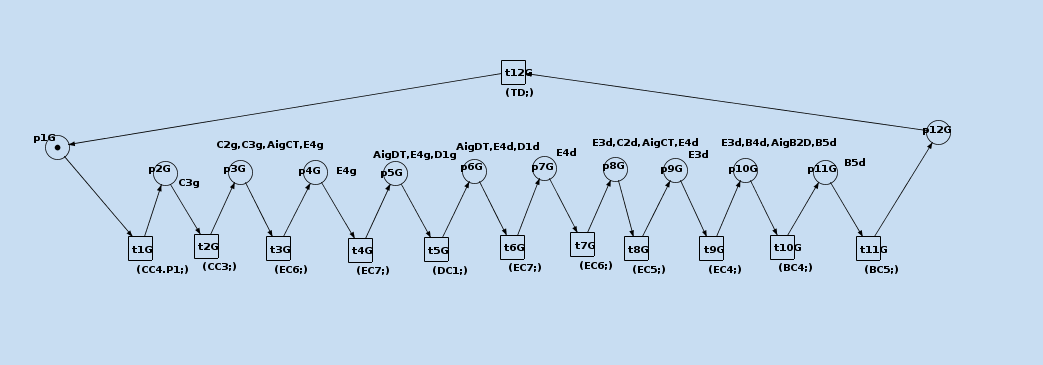
\includegraphics[width=15cm, height=7cm]{w1.png}
	\captionof{figure}{\textit{Réseau de Petri du fonctionnement d'un seul wagonnet $w1$ \\}}
	\label{fig1} 
	\end{center}
	
	\textbf{Nota:} On vous invite à zoomer sur les figures pour une meilleure clarté.  

\section{\textsc{Le code C correspondant}}

	\begin{lstlisting}
#include <stdlib.h>
#include <stdio.h>
#include <unistd.h>
#include <pthread.h>
#include "entreesortie_train.h"
#include <semaphore.h>
#include <signal.h>
#define N 6 // 6 phases charge/decharge
/*******************************************************************************


/* POUR COMPILER
/* gcc -Wall manipulation1.c -o Manipulation1 -lpthread -ltrain -lpci_dask*/

/*******************************************************************************

 /* declaration des thread et semaphores */
pthread_t train[3];
static sem_t sema;
short int idcard;

/* declaration capteurs */

unsigned char cc1=0,cc2=0,cc3=0,cc4=0,bc1=0,bc2=0,bc3=0,bc4=0,bc5=0,dc1=0;
unsigned char ec7=0, ec6=0,ec5=0,ec4=0, bp1=0, bp2=0;
unsigned char aigcd=0,aigct=0,aigb2t=0,aigb2d=0;

void stop_soft(int h) {
	printf(" ARRET par CTRL+C");
	stop=1;
}
stop=0;

// deroutement de l'IT SIGINT
signal(SIGINT, stop_soft);


// lecture des entrees
 void lectureentree()
 {

	bp1= entree(P1);
	bp2= entree(P2);
	cc1= entree(CC1);
	cc2= entree(CC2);
	cc3= entree(CC3);
	cc4= entree(CC4);
	bc5= entree(BC5);
	ec4= entree(EC4);
	ec7= entree(EC7);
	ec6= entree(EC6);
	dc1= entree(DC1);
}

void raz_sortie()
{
	sortie(B1D,0);
	sortie(B1G,0);
	sortie(B2G,0);
	sortie(B2D,0);
	sortie(B3G,0);
	sortie(B3D,0);
	sortie(B4G,0);
	sortie(B4D,0);
	sortie(B5G,0);
	sortie(B5D,0);
	sortie(C1G,0);
	sortie(C1D,0);
	sortie(C2G,0);
	sortie(C3G,0);
	sortie(C3D,0);
	sortie(D1G,0);
	sortie(D1D,0);
	sortie(D2G,0);
	sortie(D2D,0);
	sortie(D3G,0);
	sortie(D3D,0);
	sortie(E2G,0);
	sortie(E2D,0);
	sortie(E3G,0);
	sortie(E3D,0);
	sortie(E4G,0);
	sortie(E4D,0);
}

/* Codage des fonction des threads */

void *w1 (void*arg)
{
	int i;
	while(i<N) {
		while (!P1 && !cc4) {
			usleep(100);
			printf("demarrage\n",bp1);
			sortie(C2G,1);
			sortie(C3G,1);
		}
		while (!cc3) {
			usleep(100);
			printf("debut phase aller chemin 1 \n");
			sortie(aigct,1);
			sortie(C4G,1);
		}
		while (!ec6) {
			if(sortie(C4G,1)){
			usleep(100);
			sortie(aigct,0);
			sortie(C2G,0);
			sortie(C3G,0);
			printf("fin phase aller chemin 1\n");
			sortie(E4G,1);}
		}
		while (!ec7) {
			if(sortie(E4G,1)) {
			usleep(100);
			sortie(aigdt,1);
			sortie(E4G,1);
			sortie(D1G,1);}
		}
		while (!dc1) {
			usleep(100);
			sortie(E4G,0);
			sortie(D1G,0);
			printf("debut phase retour chemin 1\n");
			sortie(aigdt,1);
			sortie(E4D,1);
			sortie(D1D,1);
		}
		while (!ec7) {
			if(sortie(E4D,1)){
			usleep(100);			
			sortie(aigdt,0);
			sortie(D1D,0);
			sortie(E4D,1);}
		}
		while (!ec6) { 
			if(sortie(E4D,1)){
			usleep(100);
			sortie(E4D,1);	
			sortie(aigct,1);
			sortie(C2D,1);
			sortie(E3D,1);}
		}
		while (!ec5) {
			usleep(100);
			sortie(E4D,0);	
			sortie(aigct,0);
			sortie(C2D,0);
			sortie(E3D,1)
		}
		while (!ec4) {
			if(sortie(E3D,1)){
			usleep(100);
			sortie(E3D,1);
			sortie(aigb2d,1);
			sortie(B5D,1);
			sortie(B4D,1);}
		}
		while (!bc4) {
			if(sortie(B5D,1)){
			usleep(100);
			sortie(E3D,0);
			sortie(aigb2d,0);
			sortie(B5D,1);
			sortie(B4D,0);}
		}
		while (!bc5) { 
			usleep(100);
			sortie(B5D,0);
			printf("fin phase retour chemin 1 et debut phase de dechargement\n");
			sleep(2); //TD
			printf("fin phase de dechargement\n");
			sortie(B5G,1);
		}
		while (!bc4) {
			if(sortie(B5G,1)){ 
			printf("debut phase aller chemin 2\n");
			usleep(100);
			sortie(B5G,1);
			sortie(aigb2t,1);
			sortie(B4G,1);
			sortie(E3G,1);}
		}
		while (!ec4) {
			if(sortie(E3G,1)){
			usleep(100);
			sortie(B5G,0);
			sortie(aigb2t,0);
			sortie(B4G,0);
			sortie(E3G,1);}
		}
		while (!ec5) {
			if(sortie(E3G,1)){ 
			usleep(100);
			sortie(aigcd,1);
			sortie(E3G,1);
			sortie(C2G,1);
			sortie(C1G,1);
			sortie(E1G,0);}
		}
		while (!cc2) {
			if(sortie(C1G,1)){ 
			usleep(100);
			sortie(aigcd,0);
			sortie(E3G,0);
			sortie(C2G,0);
			sortie(C1G,1);}
		}
		while (!cc1) {
			sortie(C1G,0);
			usleep(100);
			printf("fin phase aller chemin 2\n");
			sortie(C1D,1);
		}
		while (!cc2) { 
			if(sortie(C1D,1)){
			usleep(100);
			printf("debut phase retour chemin 2");
			sortie(C1D,1);
			sortie(C2D,1);
			sortie(C3D,1);
			sortie(aigcd,1);}
		}
		while (!cc3) { 
			if(sortie(C3D,1)){
			usleep(100);
			sortie(C3D,1);
			sortie(C1D,0);
			sortie(C2D,0);
			sortie(aigcd,0);}
		}
		while (!cc4) { 
			usleep(100);
			sortie(C3D,0);
			printf("fin phase retour chemin 2 et debut phase de dechargement\n");
			sleep(2); //TD
			printf("fin phase de dechargement\n");
			sortie(C3G,1);
		}
	}
}

int main ()
{
	//int arg;
	int No;
	pthread_t Th_w1,Th_w1&w2,Th_w1&w2&w3;
	
	//intinitialisation des ports d'E/S
	init_io();
	printf("ports E/S initialisations");
	printf(" Appuyer sur touche return pour continuer");
	getchar();

	// initialisation des aiguillages
	sortie (AigCD, aigcd);
	sortie (AigCT, aigct);	
	sortie (AigB2D, aigb2d);
	sortie (AigB2T, aigb2t);
	printf(" fin intitialsation aiguillage");

	raz_sortie();
	
	/*creation des threads */
	No=pthread_create(&Th_w1,NULL,w1,"1");
	if(No!=0) {
		fprintf(stderr,"erreur a la creation du thread 1 \n");
		exit(1);
		}
		
	/* attente de la fin des threads */
	pthread_join(Th_w1,NULL);
	printf("Les threads sont terminees \n");
	
	
	//arret mise a zero de tous les actionneurs
	raz_sortie();
	Release_Card(idcard);
	return 0;
}
	\end{lstlisting}

%%%%%%%%%%%%%%%%%%%%%
	
\chapter{\textsc{ Modélisation du fonctionnement de deux wagonnets $w1$ et $w2$ }}
\section{\textsc{Le réseau de Petri}}
	
	\begin{center}
	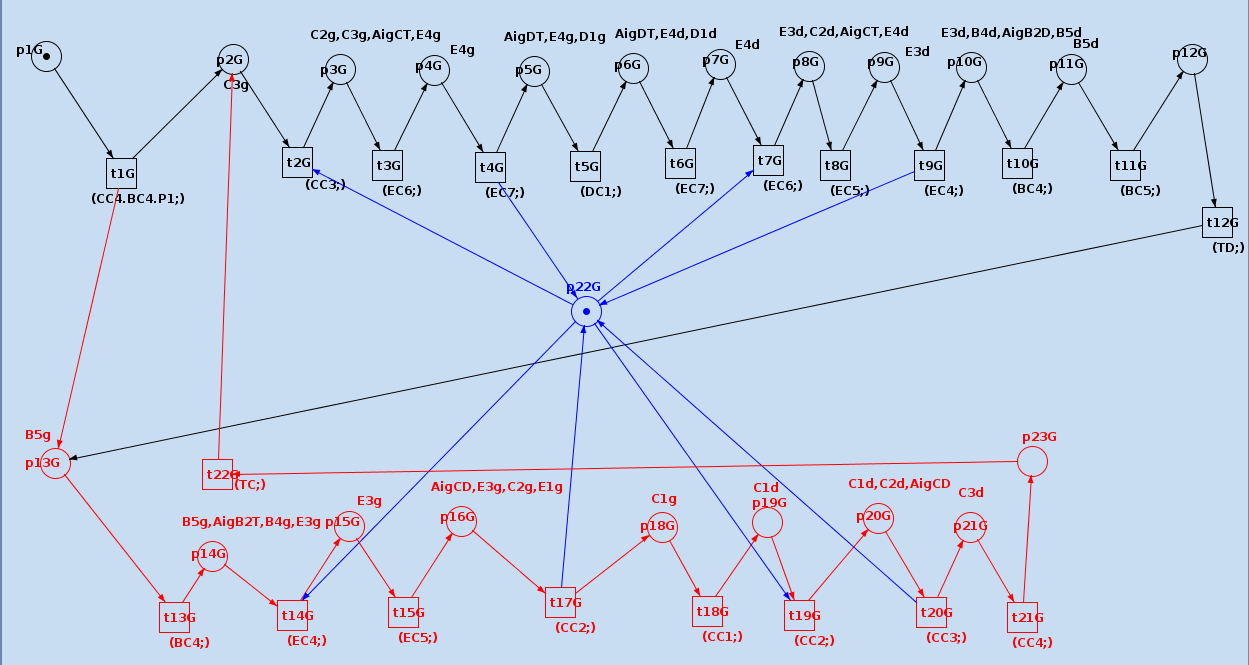
\includegraphics[width=15cm, height=10cm]{w2.png}
	\captionof{figure}{\textit{Réseau de Petri du fonctionnement de deux wagonnets $w1$ et $w2$ \\}}
	\label{fig2} 
	\end{center} 
	\par Le chemin en noir représente la phase du déchargement ds wagonnets $w1$ et $w2$  suivi du chemin  en rouge qui représente la phase de chargement. La partie bleue représente la gestion de la resource partagée entre $w1$ et $w2$ qu'on a réduit au canton $C2$.  

\section{\textsc{Le code C correspondant}}

	\begin{lstlisting}
#include <stdlib.h>
#include <stdio.h>
#include <unistd.h>
#include <pthread.h>
#include "entreesortie_train.h"
#include <semaphore.h>
#include <signal.h>
#define N 13 // 13 phases charge/decharge
/*******************************************************************************


/* POUR COMPILER
/* gcc -Wall manipulation1.c -o Manipulation1 -lpthread -ltrain -lpci_dask*/

/*******************************************************************************

 /* declaration des thread et semaphores */
pthread_t train[3];
static sem_t sema;
short int idcard;

/* declaration capteurs */

unsigned char cc1=0,cc2=0,cc3=0,cc4=0,bc1=0,bc2=0,bc3=0,bc4=0,bc5=0,dc1=0;
unsigned char ec7=0, ec6=0,ec5=0,ec4=0, bp1=0, bp2=0;
unsigned char aigcd=0,aigct=0,aigb2t=0,aigb2d=0;

void stop_soft(int h) {
	printf(" ARRET par CTRL+C");
	stop=1;
}
stop=0;

// deroutement de l'IT SIGINT
signal(SIGINT, stop_soft);


// lecture des entrees
 void lectureentree()
 {

	bp1= entree(P1);
	bp2= entree(P2);
	cc1= entree(CC1);
	cc2= entree(CC2);
	cc3= entree(CC3);
	cc4= entree(CC4);
	bc5= entree(BC5);
	ec4= entree(EC4);
	ec7= entree(EC7);
	ec6= entree(EC6);
	dc1= entree(DC1);
}

void raz_sortie()
{
	sortie(B1D,0);
	sortie(B1G,0);
	sortie(B2G,0);
	sortie(B2D,0);
	sortie(B3G,0);
	sortie(B3D,0);
	sortie(B4G,0);
	sortie(B4D,0);
	sortie(B5G,0);
	sortie(B5D,0);
	sortie(C1G,0);
	sortie(C1D,0);
	sortie(C2G,0);
	sortie(C3G,0);
	sortie(C3D,0);
	sortie(D1G,0);
	sortie(D1D,0);
	sortie(D2G,0);
	sortie(D2D,0);
	sortie(D3G,0);
	sortie(D3D,0);
	sortie(E2G,0);
	sortie(E2D,0);
	sortie(E3G,0);
	sortie(E3D,0);
	sortie(E4G,0);
	sortie(E4D,0);
}

/* Codage des fonction des threads */

void *w1&w2 (void*arg)
{
	int i;
	while(i<N) {
		while (!P1 && !cc4 && !bc4) {
			usleep(100);
			printf("demarrage\n",bp1);
			sortie(C2G,1);
			sortie(C3G,1);
		}
		while (!cc3) {
			usleep(100);
			printf("debut phase aller chemin 1 \n");
			sem_wait(&sema);
			sortie(aigct,1);
			sortie(C4G,1);
		}
		while (!ec6) {
			if(sortie(C4G,1)){
			usleep(100);
			sortie(aigct,0);
			sortie(C2G,0);
			sortie(C3G,0);
			printf("fin phase aller chemin 1\");
			sortie(E4G,1);}
		}
		while (!ec7) {
			if(sortie(E4G,1)) {
			usleep(100);
			sem_post(&sema);
			sortie(aigdt,1);
			sortie(E4G,1);
			sortie(D1G,1);}
		}
		while (!dc1) {
			usleep(100);
			sortie(E4G,0);
			sortie(D1G,0);
			printf("debut phase retour chemin 1\n");
			sortie(aigdt,1);
			sortie(E4D,1);
			sortie(D1D,1);
		}
		while (!ec7) {
			if(sortie(E4D,1)){
			usleep(100);			
			sortie(aigdt,0);
			sortie(D1D,0);
			sortie(E4D,1);}
		}
		while (!ec6) { 
			if(sortie(E4D,1)){
			usleep(100);
			sem_wait(&sema);
			sortie(E4D,1);	
			sortie(aigct,1);
			sortie(C2D,1);
			sortie(E3D,1);}
		}
		while (!ec5) {
			usleep(100);
			sortie(E4D,0);	
			sortie(aigct,0);
			sortie(C2D,0);
			sortie(E3D,1)
		}
		while (!ec4) {
			if(sortie(E3D,1)){
			usleep(100);
			sem_post(&sema);
			sortie(E3D,1);
			sortie(aigb2d,1);
			sortie(B5D,1);
			sortie(B4D,1);}
		}
		while (!bc4) {
			if(sortie(B5D,1)){
			usleep(100);
			sortie(E3D,0);
			sortie(aigb2d,0);
			sortie(B5D,1);
			sortie(B4D,0);}
		}
		while (!bc5) { 
			usleep(100);
			sortie(B5D,0);
			printf("fin phase retour chemin 1 et debut phase de dechargement\n");
			sleep(2); //TD
			printf("fin phase de dechargement\n");
			sortie(B5G,1);
		}
		while (!bc4) {
			if(sortie(B5G,1)){ 
			printf("debut phase aller chemin 2\n");
			usleep(100);
			sortie(B5G,1);
			sortie(aigb2t,1);
			sortie(B4G,1);
			sortie(E3G,1);}
		}
		while (!ec4) {
			if(sortie(E3G,1)){
			usleep(100);
			sem_wait(&sema);
			sortie(B5G,0);
			sortie(aigb2t,0);
			sortie(B4G,0);
			sortie(E3G,1);}
		}
		while (!ec5) {
			if(sortie(E3G,1)){ 
			usleep(100);
			sortie(aigcd,1);
			sortie(E3G,1);
			sortie(C2G,1);
			sortie(C1G,1);
			sortie(E1G,0);}
		}
		while (!cc2) {
			if(sortie(C1G,1)){ 
			usleep(100);
			sem_post(&sema);
			sortie(aigcd,0);
			sortie(E3G,0);
			sortie(C2G,0);
			sortie(C1G,1);}
		}
		while (!cc1) {
			sortie(C1G,0);
			usleep(100);
			printf("fin phase aller chemin 2\n");
			sortie(C1D,1);
		}
		while (!cc2) { 
			if(sortie(C1D,1)){
			usleep(100);
			sem_wait(&sema);
			printf("debut phase retour chemin 2");
			sortie(C1D,1);
			sortie(C2D,1);
			sortie(C3D,1);
			sortie(aigcd,1);}
		}
		while (!cc3) { 
			if(sortie(C3D,1)){
			usleep(100);
			sem_post(&sema);
			sortie(C3D,1);
			sortie(C1D,0);
			sortie(C2D,0);
			sortie(aigcd,0);}
		}
		while (!cc4) { 
			usleep(100);
			sortie(C3D,0);
			printf("fin phase retour chemin 2 et debut phase de dechargement\n");
			sleep(2); //TD
			printf("fin phase de dechargement\n");
			sortie(C3G,1);
		}
	}
}

int main ()
{
	//int arg;
	int No;
	pthread_t Th_w1,Th_w1&w2,Th_w1&w2&w3;
	
	//intinitialisation des ports d'E/S
	init_io();
	printf("ports E/S initialisations");
	printf(" Appuyer sur touche return pour continuer");
	getchar();

	// initialisation des aiguillages
	sortie (AigCD, aigcd);
	sortie (AigCT, aigct);	
	sortie (AigB2D, aigb2d);
	sortie (AigB2T, aigb2t);
	printf(" fin intitialsation aiguillage");

	// initialisation des semaphores
	sem_init(&sema,1,0);
	raz_sortie();
	
	/*creation des threads */
	No=pthread_create(&Th_w1&w2,NULL,w1&w2,"1");
	if(No!=0) {
		fprintf(stderr,"erreur a la creation du thread 2 \n");
		exit(1);
	}

	/* attente de la fin des threads */
	
	pthread_join(Th_w1&w2,NULL);
	//pthread_join(e1_lectureentree,NULL);
	printf("Les threads sont terminees \n");
	fflush(stdout);
	
	//arret mise a zero de tous les actionneurs
	raz_sortie();
	Release_Card(idcard);
	return 0;
}
	\end{lstlisting}


%%%%%%%%%%%%%%%%%%%%%

\chapter{\textsc{ Modélisation du fonctionnement des trois wagonnets $w1$, $w2$ et $w3$}}
\section{\textsc{Le réseau de Petri}}
	
	\begin{center}
	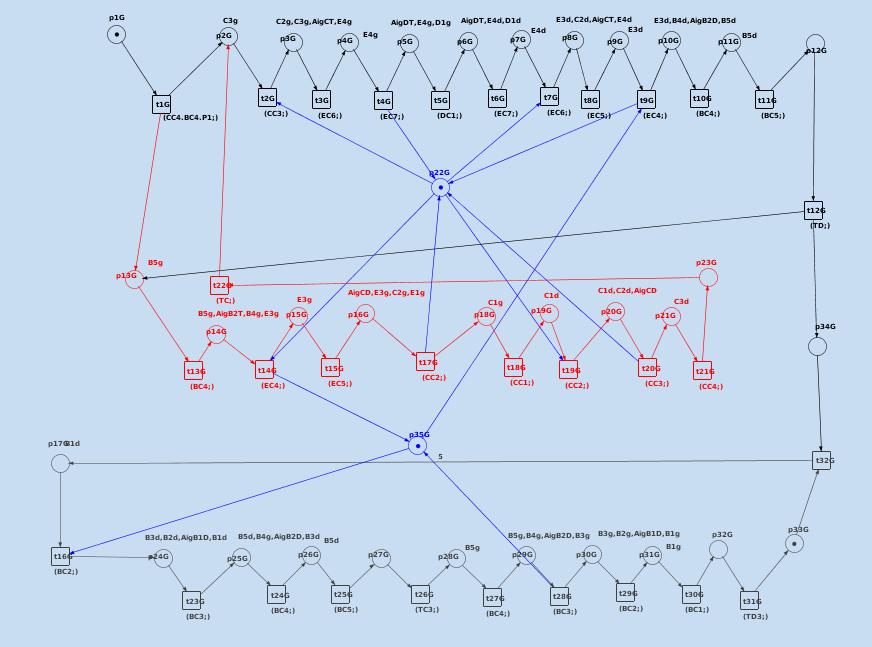
\includegraphics[width=15cm, height=10cm]{w3.png}
	\captionof{figure}{\textit{Réseau de Petri du fonctionnement des tros wagonnets $w1$, $w2$ et $w3$ \\}}
	\label{fig3} 
	\end{center}  

%%%%%%%%%%%%%%%%%%

\chapter*{\textsc{Conclusion}}
\addcontentsline{toc}{chapter}{\textsc{Conclusion}}

	\paragraph{} Nous n'avons pas pu terminer la dernière partie de cette séance, ni de tester la maquette à défaut de temps. Mais nous avons appris à modéliser puis à coder proprement un système parallèle complexe. Avec un débogage nous avons pu couriger nos erreurs et nous avons réussi à simuler sans avoir de problème.\\